
\documentclass[journal]{IEEEtran}
% *** MISC UTILITY PACKAGES ***
%\usepackage{ifpdf}

% *** CITATION PACKAGES ***
%\usepackage{cite}

% *** GRAPHICS RELATED PACKAGES ***
\ifCLASSINFOpdf
  \usepackage[pdftex]{graphicx}
  % declare the path(s) where your graphic files are
  \graphicspath{{PDF/}}
  % and their extensions so you won't have to specify these with
  % every instance of \includegraphics
  \DeclareGraphicsExtensions{.pdf}
\else
  % \usepackage[dvips]{graphicx}
  % declare the path(s) where your graphic files are
  % \graphicspath{{../eps/}}
  % and their extensions so you won't have to specify these with
  % every instance of \includegraphics
  % \DeclareGraphicsExtensions{.eps}
\fi

% *** MATH PACKAGES ***
%\usepackage{amsmath}
% Note that the amsmath package sets \interdisplaylinepenalty to 10000
% thus preventing page breaks from occurring within multiline equations. Use:
%\interdisplaylinepenalty=2500

% *** SPECIALIZED LIST PACKAGES ***
%\usepackage{algorithmic}

% *** ALIGNMENT PACKAGES ***
%\usepackage{array}

% *** SUBFIGURE PACKAGES ***
%\ifCLASSOPTIONcompsoc
%  \usepackage[caption=false,font=normalsize,labelfont=sf,textfont=sf]{subfig}
%\else
%  \usepackage[caption=false,font=footnotesize]{subfig}
%\fi

% *** FLOAT PACKAGES ***
%\usepackage{fixltx2e}
% Be aware that LaTeX2e kernels dated 2015 and later have fixltx2e.sty's
% corrections already built into the system in which case a warning will
% be issued if an attempt is made to load fixltx2e.sty as it is no longer
% needed.

%\usepackage{stfloats}
%\fnbelowfloat
% to enable the placement of footnotes below bottom floats (the standard
% LaTeX2e kernel puts them above bottom floats). This is an invasive package
% which rewrites many portions of the LaTeX2e float routines. It may not work
% with other packages that modify the LaTeX2e float routines.

% Do not attempt to use stfloats with fixltx2e as they are incompatible.
% Instead, use Morten Hogholm'a dblfloatfix which combines the features
% of both fixltx2e and stfloats:
% \usepackage{dblfloatfix}

%\ifCLASSOPTIONcaptionsoff
%  \usepackage[nomarkers]{endfloat}
% \let\MYoriglatexcaption\caption
% \renewcommand{\caption}[2][\relax]{\MYoriglatexcaption[#2]{#2}}
%\fi

% *** PDF, URL AND HYPERLINK PACKAGES ***
\usepackage{url}
% Basically, \url{my_url_here}.

% correct bad hyphenation here


\begin{document}
\title{StreamGraph Documentation\\KBS Projekt}
\author{Florian~Ziesche, Jakob~Karge and Boris~Graf\\TU-Berlin\\2016}

% The paper headers
\markboth{StreamGraph Documentation}%
{StreamGraph Documentation}

% use for special paper notices%\begin{figure}[!t]
%\centering
%\includegraphics[width=2.5in]{myfigure}
%\caption{Simulation results for the network.}
%\label{fig_sim}
%\end{figure}
%\IEEEspecialpapernotice{(Invited Paper)}

\maketitle

\begin{abstract}
The abstract goes here.
\end{abstract}


\section{Introduction}
\IEEEPARstart{T}{he} StreamGraph project aims to present the StreamIt language
simplified in a graphical environment. As such it is intended to be used by
people who have little programming experience or do not wish to engage with the
specifics of the StreamIt language and alleviates the amount of StreamIt
specific semantic knowledge. StreamGraph does not contain every construct
or possibility that StreamIt provides since it does not aim to rebuild the
language in a graphical environment.



\subsection{StreamIt Language}
\noindent StreamIt is a language specifically build for applications which
process a continuous stream of data. To achieve good performance on multi-core
or multi-processor machines StreamIt enables highly parallel programming and
programs, while trying to keep the programming as simple as possible.\\

The language features specific basic modules. This documentation focuses on the
StreamGraph project and so only the subset of StreamIt modules which are
realized in StreamGraph today are included and briefly explained. For further
documentation on StreamIt see \cite{streamIt}.\\

The most basic module of the StreamIt language and the only module that
processes data is the filter. A filter, just as any other StreamIt construct,
has exactly one input and exactly one output for data. It consists mainly of 
an init and a work function. The init function describes the filter's initial
condition (e.g. initial values of variables). The work function describes the
steps taken in one execution step of the filter and is called every time that
the preconditions are fulfilled.\\

These preconditions are described by the pop, peek and push values. The pop
value describes how many data packages are taken from the input of the filter in
a single execution step of the work function. Similarly the pop value describes
how many data packages are produced in the output of the filter in that
execution step. The peek value describes how far back the filter needs to read
in the input data, i.e. the minimum input queue length, since any value read has
to be processed by previous filters.


\subsubsection{StreamIt topology}
\label{StreamItTopology}
\noindent Since filters alone do not specify in which order and if they are
connected it is necessary to have language constructs which describe the
connections and the structure of the processing. These constructs will be
referred to as topological construct in the further documentation.\\

One of these constructs is the pipeline. A pipeline connects filters, pipelines
and split-join constructs in a linear fashion. Each pipline has an init function
in which the elements of the pipeline are added and which determines the order
in which a datapacket is processed. Agraphical representation of a pipeline can 
be seen in fig. \ref{fig_Pipeline}.\\
\\

\begin{figure}[h]
	\centering
	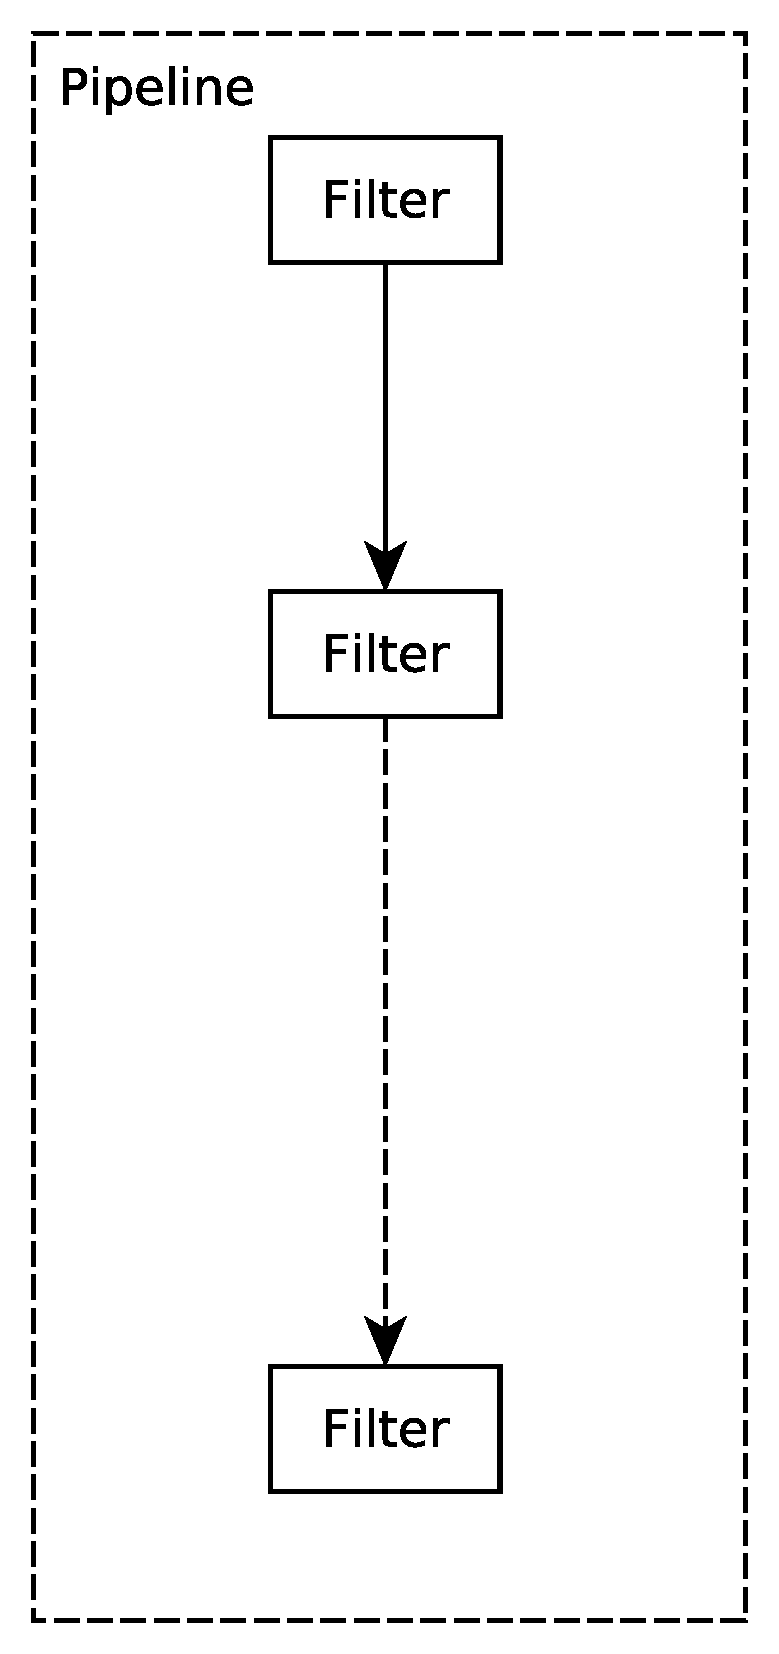
\includegraphics[width=0.3\textwidth]{PipelineGraphic}
	\caption{Example of a pipeline}
	\label{fig_Pipeline}
\end{figure}


\noindent The second construct supported by StreamGraph is the split-join construct. 
This constucts splits the data packets of its input to multiple data paths on which
other constructs are placed and joins these paths together at the end of every
path. All in all a split-join construct has exactly one input and one output, as can 
be seen in fig. \ref{fig_Split_Join}.\\
\\

\begin{figure}[h]
	\centering
	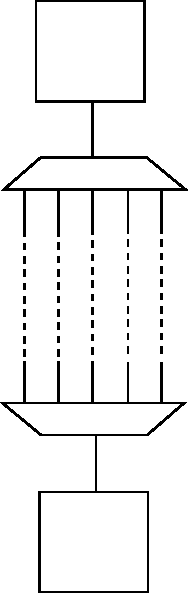
\includegraphics[width=0.3\textwidth]{SplitJoinGraphic}
	\caption{Example of a split-join construct}
	\label{fig_Split_Join}
\end{figure}


\noindent The StreamIt language generates a pipeline based structure. As such
it is not possible to connect two filters or constructs in different pipelines (see Fig.
\ref{fig_StreamIt_topology}.).\\
\begin{figure}[h]
	\centering
	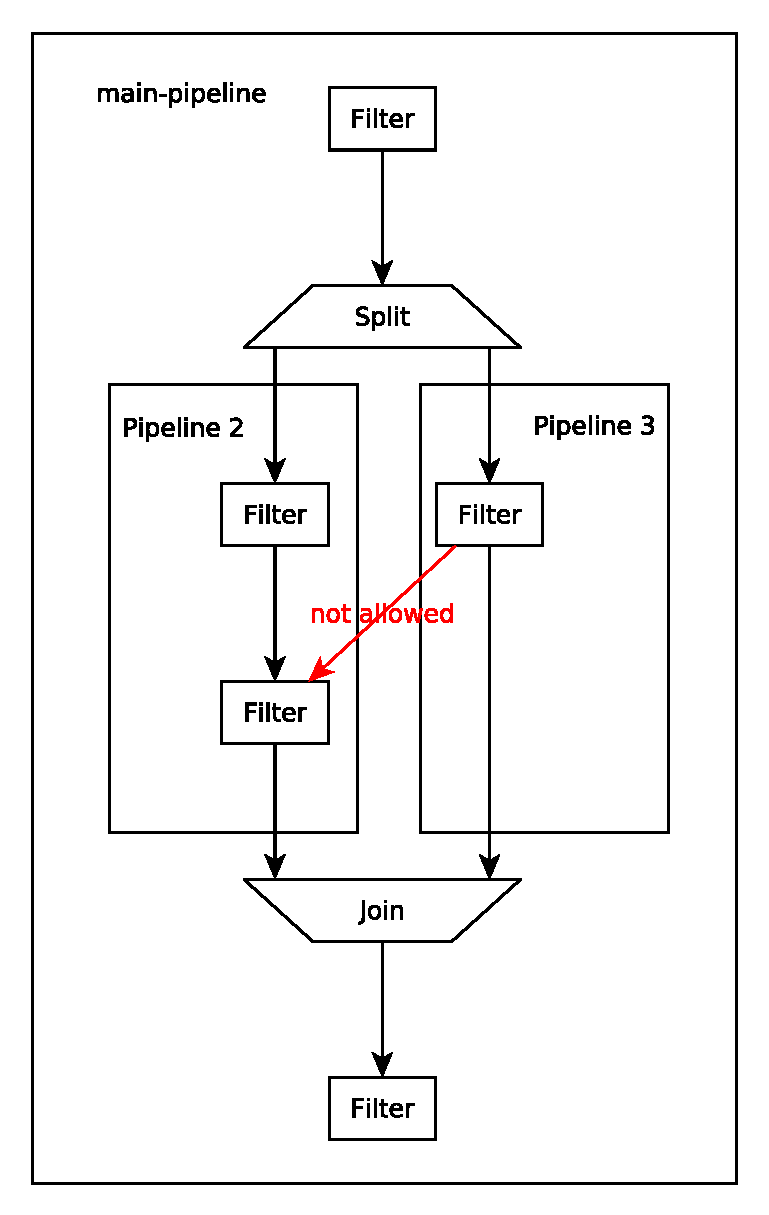
\includegraphics[width=0.4\textwidth]{StreamItTopology}
	\caption{Example for a non permissable connection between pipelines}
	\label{fig_StreamIt_topology}
\end{figure}
\noindent Since split-join constructs have exactly one input and one output and only appear in pairs it is not
 possible to have connections from one split-join pair to another pair(see Fig.
 \ref{fig_StreamIt_topology_between_SJ}) or to have an unequal numbers of splits and joins (see Fig.
 \ref{fig_StreamIt_topology_missing_join}).\\
\begin{figure}[h]
	\centering
	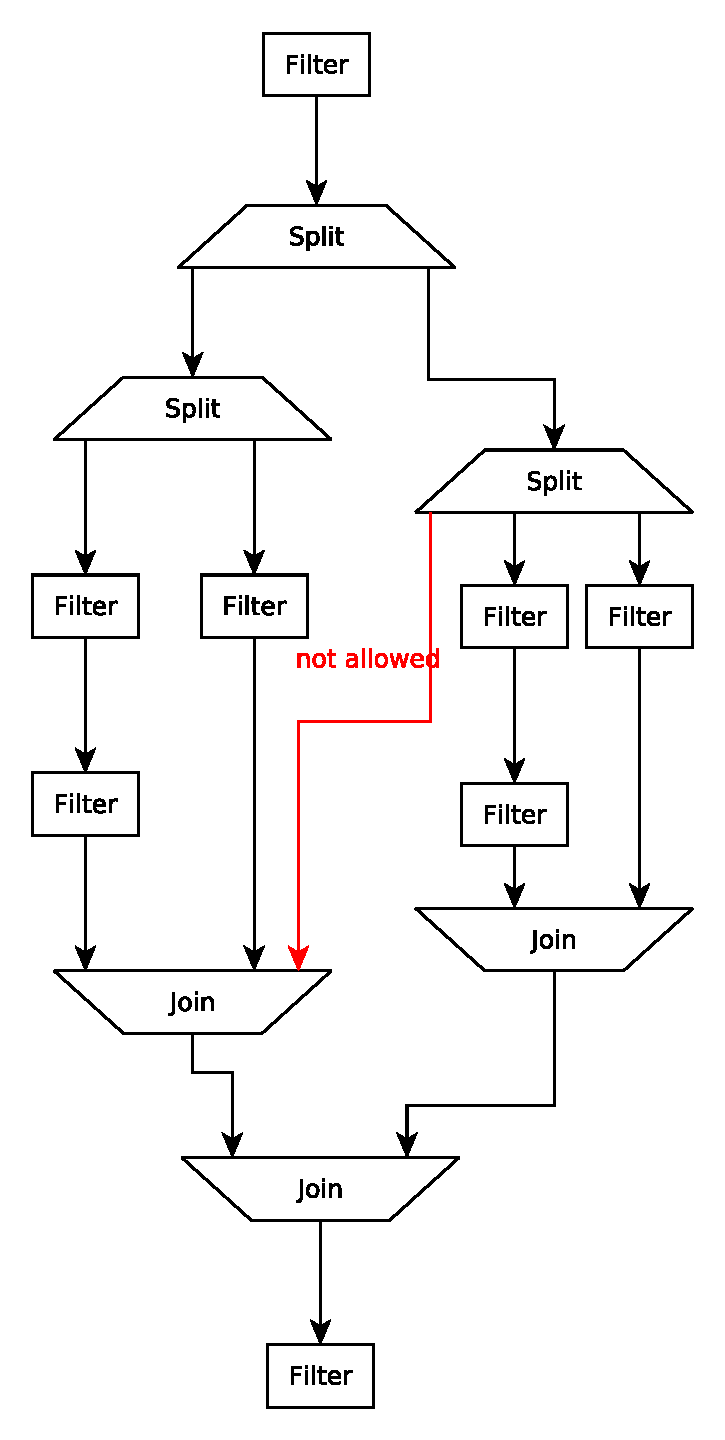
\includegraphics[width=0.4\textwidth]{StreamItTopologyBetweenSJ}
	\caption{Example for a non permissable connection between split-join pairs}
	\label{fig_StreamIt_topology_between_SJ}
\end{figure}
\begin{figure}[h]
	\centering
	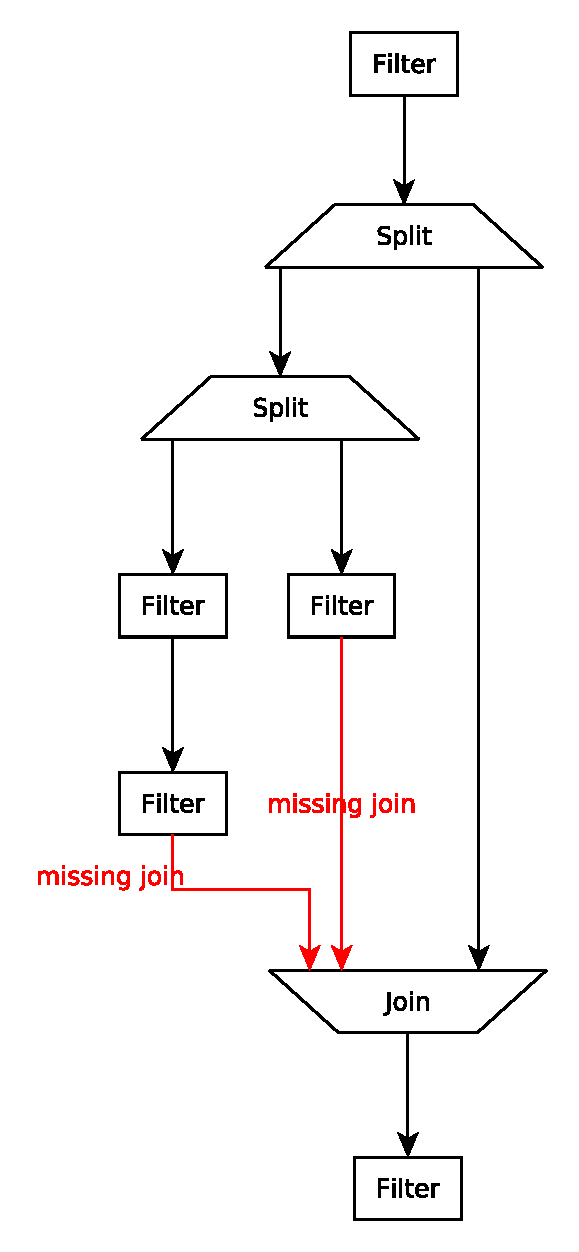
\includegraphics[width=0.4\textwidth]{StreamItTopologyMissingJoin}
	\caption{Example for a unequal number of splits and joins (in this case a missing join)}
	\label{fig_StreamIt_topology_missing_join}
\end{figure}
% needed in second column of first page if using \IEEEpubid
%\IEEEpubidadjcol


\section{StreamGraph}

\noindent The StreamGraph project is composed of multiple parts. In this
section they are listed and explained and along with the reason behind the
individual decisions that led to them.

\subsection{View}
\noindent The GUI of StreamGraph includes three parts. At the top is the menu
bar with the important functions for the project. The first submenu is, similar to
other textual editors, the File menu with common functions to create new, open, save,
save-as or to quit projects. In the Edit submenu it is possible to create new objects.
In the Run submenu the project can be executed. The Debug submenu helps with debugging
the project. \\

% http://search.cpan.org/~hemlock/Gtk2-Ex-MindMapView-0.000001/lib/Gtk2/Ex/MindMapView.pm
The view takes up the main part of the GUI window. It is based on the Gtk2::Ex::MindMapView
Perl modul \cite{GTK2EXMindMapView} and shows the objects and their connections. The view design
is minimalistic: a plain surface to have a clear view and simple usability.
There are no toolbars or other control windows. The graph structure
can be completely edited with the mouse. A right click opens a pop-up menu with the
same entries as in the Edit submenu. This allows the creation of an object with two mouse
clicks. The surface can be scrolled with the scrollbars in all four directions,
but can also be dragged with the left mouse button. It gives the user access to a larger
editing area and to seperate objects into different groups. \\

At the bottom of the GUI is a dynamic status bar for program feedback for the user.
Errors or important information are shown there. \\

\subsubsection{Objects}
Objects wich are shown on the view surface are nodes of the program graph. There
are four different types: Filter, Parameter, Subgraph and Comment. Each type has
a different geometric form. Connections between the nodes are visualized as lines
with a direction arrow. Connections have circular pins at both the beginnig and the end.
Pins on nodes with no connection line show that this node has an open input or output.
A new connection is created by clicking on an out pin and dragging to another node.
All possible connections are visualized with bigger pins. If the mouse hovers over a
node to which the connection is possible, the arrow is glued to the available pin. \\

A connection can be marked through hovering over it with the mouse. This is visualized with a much
thicker line. A node can be marked with a left mouse click. To mark more than one
node a right mouse click on a node adds the node to the marked nodes. Another intuitive
way is to draw a selection rectangle with a right mouse click on the view surface.
Marked objects can be deleted with a DEL key press. \\

\subsubsection{Property Window}
A double left click on a node opens its property window. It contains all the parameters
from this node. For example a filter node has three tabs: Join, Filter and Split.
In the filter tab the user has the possibility to set the input and output types and
also to edit the filter source code.


\subsection{Model}

\noindent The StreamGraph layer on top of StreamIt needs data structures to
work with. Their details contain much of the design of StreamGraph as an
abstraction over StreamIt. The various data objects of StreamGraph are now
examined in further detail:

\subsubsection{Filter}
\begin{figure}[h]
  \centering
  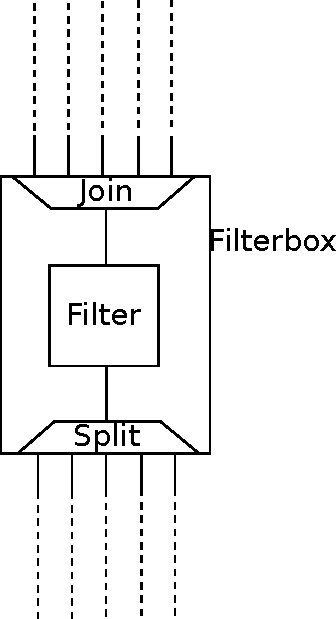
\includegraphics[width=0.2\textwidth]{FilterBoxGraphic}
  \caption{A node in the StreamGraph}
  \label{fig_filter_node}
\end{figure}

A filter in StreamGraph is a combination of two StreamIt constructs, the
filter and split-join constructs. The combination of the two into one object
has one important advantage: It allows filters to have more than one input or
output. The filter part is a very straight wrapper around a StreamIt filter,
with all the fields exposed in the property window, and a direct assembly into
a StreamIt filter on code generation.

The split-join part however is reversed and a StreamGraph filter includes a
join before and a split after. This way the multiple inputs of a filter in
StreamGraph are joined to form the required single input for a StreamIt
filter. Similarly the data packages coming from the single output of the
filter code are spread among the outputs of the StreamGraph filter node. The
join and split is configured through the filter's property window, along with
the filter code.

\subsubsection{Subgraph}

Subgraphs are slightly special in that they open another .sigraph file for
inclusion in the program. From the outside though they behave just like normal
filters and have the same properties and can be used the same way. They
encapsulate StreamIt code in a similar way that functions or methods in
textual code do.

Currently there are limits to their implementation though:

\begin{itemize}

\item Changes aren't reflected in code generation until saved.

\item No synchronization between multiple instances/windows of the same subgraph.

\item Parameters connected to subgraphs are forwarded to \emph{all} nodes in
the subgraphs, including sub-subgraphs, leading to a lot of potentially
unnecessary parameter connections.

\end{itemize}

\subsubsection{Parameter}

A parameter is a single static named value that can be used by filters (and
subgraphs) and is independent of the data stream. Its significance lies in the
use for a DRY programming style.

\subsubsection{Comment}

A comment is an inactive, unconnectable node that allows to place text
anywhere on the canvas and thus to document the code rather freely, or to
otherwise help in understanding the program.



\subsection{Graph hierarchy and Namespaces}

\noindent StreamGraph introduces Subgraphs as a new feature for structuring
code. Subgraphs act like normal filter nodes in the parent graph, but are
actually a pipeline. This makes use of the fact that pipelines and filters can
be used in the same context in StreamIt, namely in other pipelines and in
split-join constructs.

The passing of parameters down through a subgraph hierarchy makes the use of
namespaces necessary. These are fully automatic though and the user has no
interaction with them. Any parameters in a subgraph are prepended with the
name of the subgraph, to differentiate it from possibly identically named
parameters being passed in from the parent graph.



\subsection{GraphCompat}

\noindent The StreamIt topology, as discussed in \ref{StreamItTopology}, is not
only a directed Graph but has additional restrictions. Some of these are not
strictly necessary and some effort was made in StreamGraph to allow for graphs
that are not strictly StreamIt-compatible and to automatically convert them.

This task is taken on by the GraphCompat class. It transforms a given
StreamGraph graph, coming from the user interface, into a new graph which
is compatible with the StreamIt topology.

At the moment it takes care of the following 3 transformations:

\begin{itemize}
\item Identities\\
  StreamIt does not allow direct connections between a split and a join without
  a filter or a pipeline. In StreamGraph such a connection is allowed. In this
  case GraphCompat adds an identity filter instead of the direct connection
  between the split and the join, as can be seen in Fig.
  \ref{fig_split_join_identity}. This filter copies his input to his output
  without changing the content in any way.\\

\begin{figure*}[h]
	\centering
	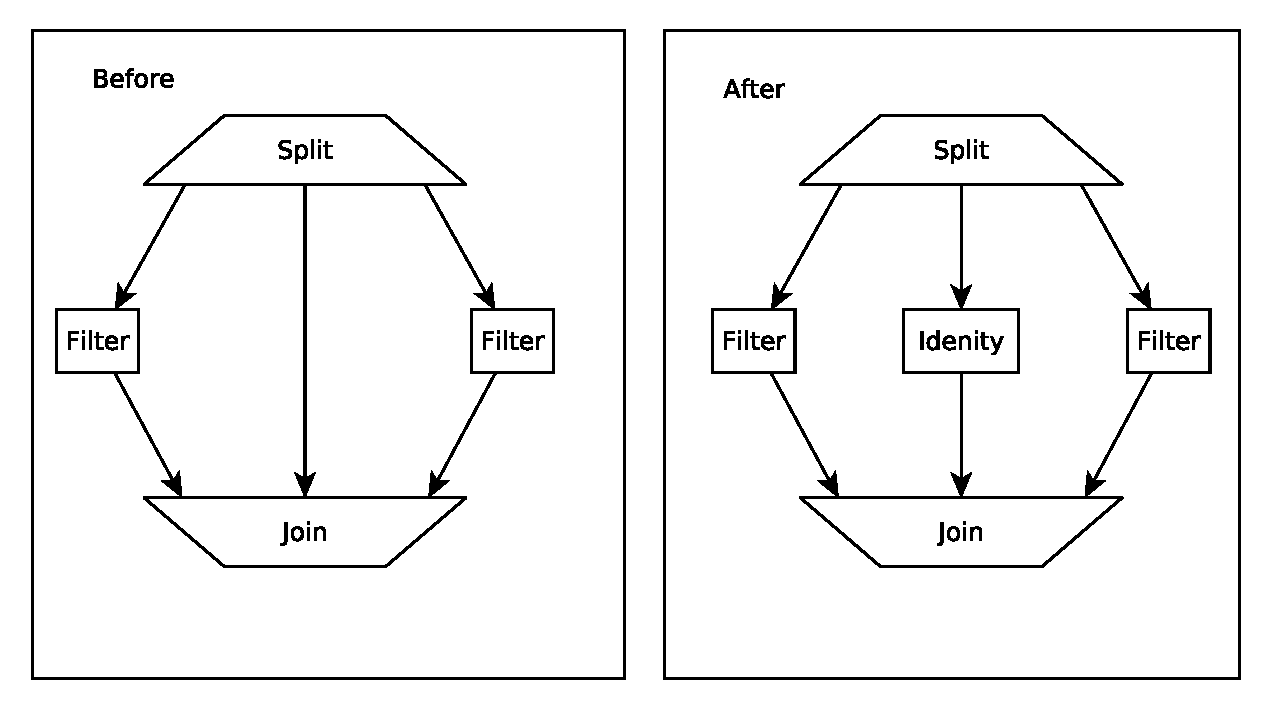
\includegraphics[width=0.8\textwidth]{SplitJoinIdentity}
	\caption{Example of adding an identity filter}
	\label{fig_split_join_identity}
\end{figure*}

\item Sources and Sinks\\
  A StreamIt graph must start and end with exactly one void-typed input and
  output respectively. StreamGraph also makes the void-typed requirement but
  does not restrict the graph to just one source and one sink. Multiple sources
  and sinks are combined by adding "Void Sources" and "Void Sinks" to the ends
  of the graph when necessary. See Fig. \ref{fig_void_end} for an illustration
  of this.\\

\begin{figure*}[h]
	\centering
	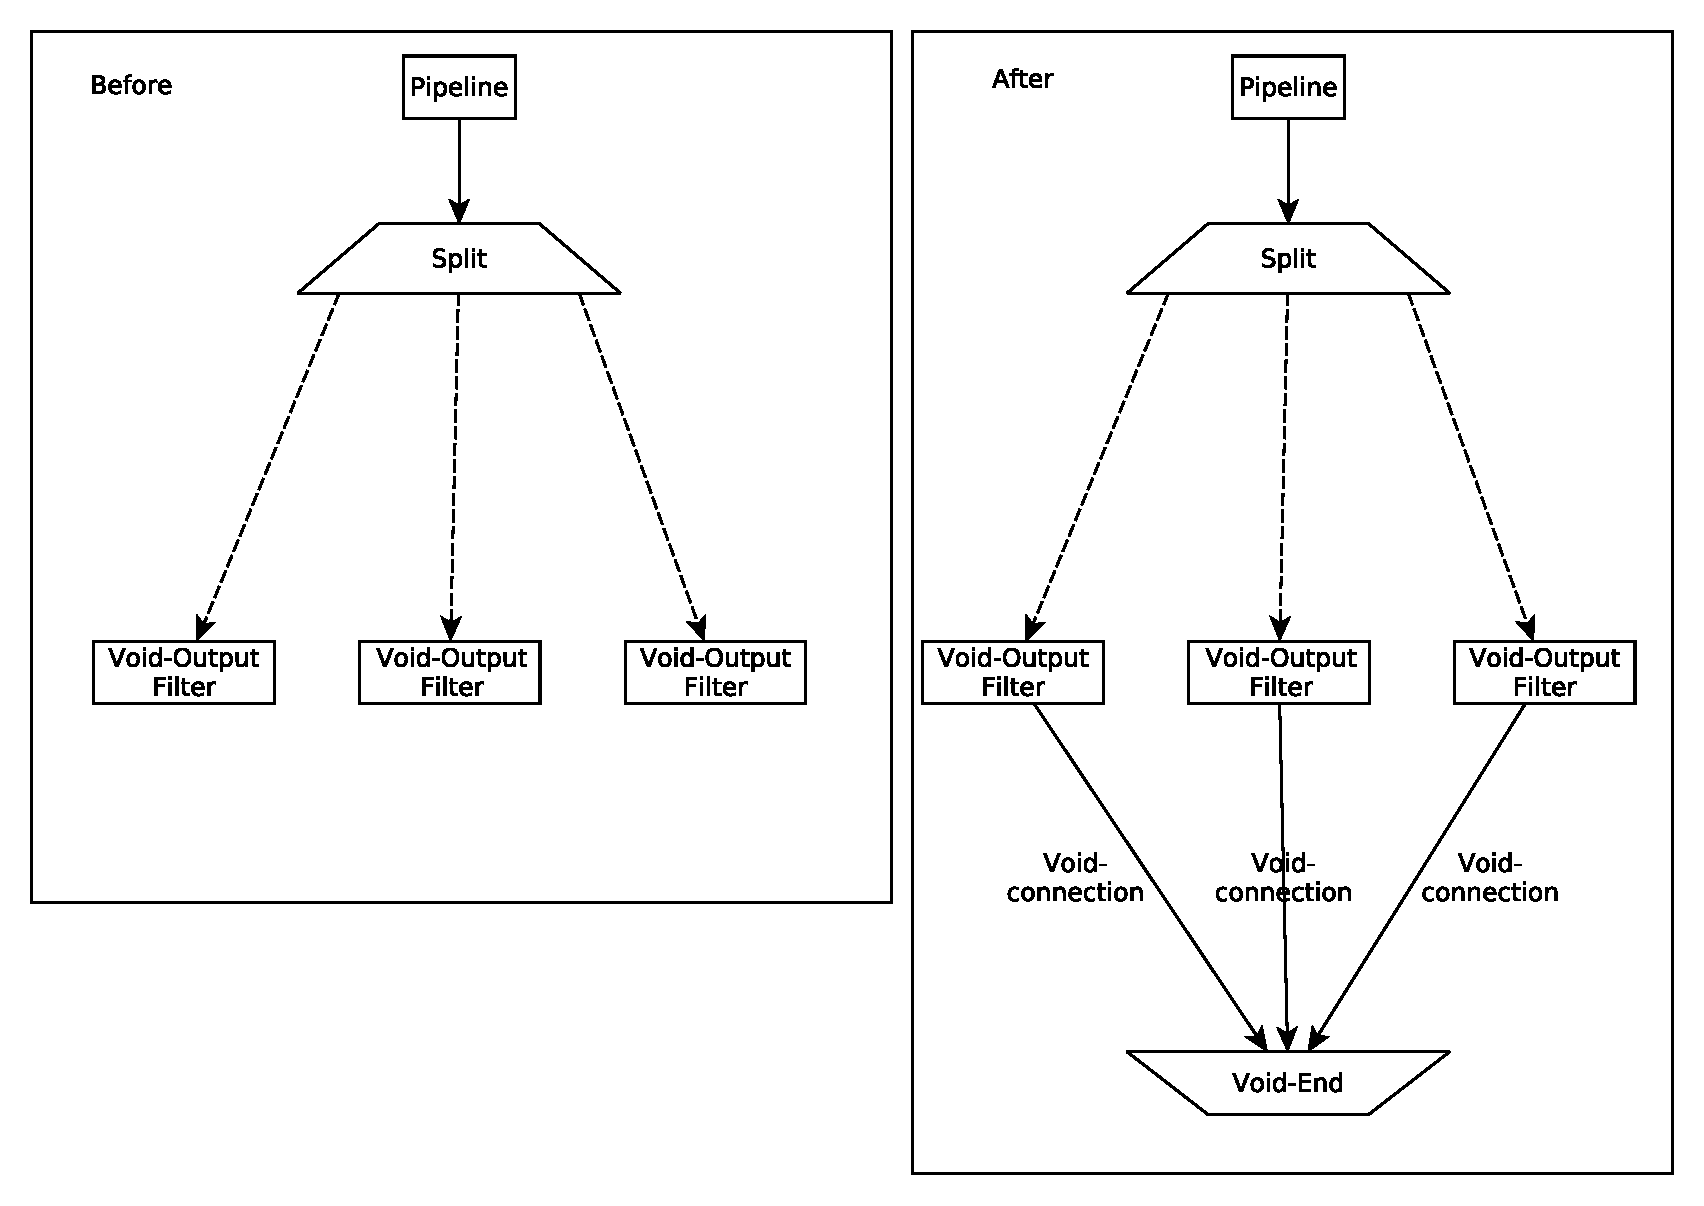
\includegraphics[width=\textwidth]{VoidEnd}
	\caption{Example of adding a void-end}
	\label{fig_void_end}
\end{figure*}

\item Subgraphs\\
  Subgraphs as they are, are a feature of StreamGraph, and don't make use of
  StreamIt's joint-compilation features. The results are essentially the same
  though: Flattening the graph hierarchy into one single graph is possible
  because a subgraph is a pipeline and using a subgraph is identical to adding
  a pipline inline.\\
  The subgraph transformation also takes care of namespacing the parameters as
  discussed above.\\

\end{itemize}

If, for one reason or another, the a part of the graph cannot be transformed
it is simply left out of the transformed graph and thus code generation. This
feature is quite essential, because otherwise a quick draft on the side of a
few nodes would quickly invalidate the whole program. But being able to test
the program as far as possible during development is necessary for a more
robust process.


\subsection{CodeObject}
\noindent The CodeObject is an interface class which is extended by the Pipeline
class, the SplitJoin class and the Parameter class. It is a general class for
all implemented topological constructs of the StreamIt language. Filters are not
CodeObjects since they do not describe the structure of the graph but rather are
the nodes of the Graph.\\
While Parameters also do not describe the structure of the graph, they may be
needed by multiple CodeObjects and are needed in different configurations while
the code is generated. As such the parameters are an exception to the general
rule that CodeObjects describe the structure of the graph. CodeObjects except
for parameters reference to other CodeObjects or filters. As such a single
CodeObject can have an entire graph ready for code generation stored in a manner
that already has the necessary order and hierarchical structure of a StreamIt
program.\\
Since StreamGraph does not use the concepts of pipelines and split-joines in 
the way StreamIt expects these constructs the codeObjects rebuild the graph 
with pipeplines and split-joines in a indirect recursive fashion, that 
resembles StreamIt's own way of nesting split-joines and pipelines into 
each other. At the same time this is the reason for creating the 
codeObjects in this way, since it automaticly generates the needed 
and desired hierarchical structure of a StreamIt program. This 
simplifies the generation of the code for a specific codeObject, 
which demands the names of all directly nested codeObjects.\\
Figure \ref{fig_StreamGraph_To_StreamIt} shows an example of a 
conversion from a simple StreamGraph graph to a CodeObject structure.\\

\begin{figure*}[h]
	\centering
	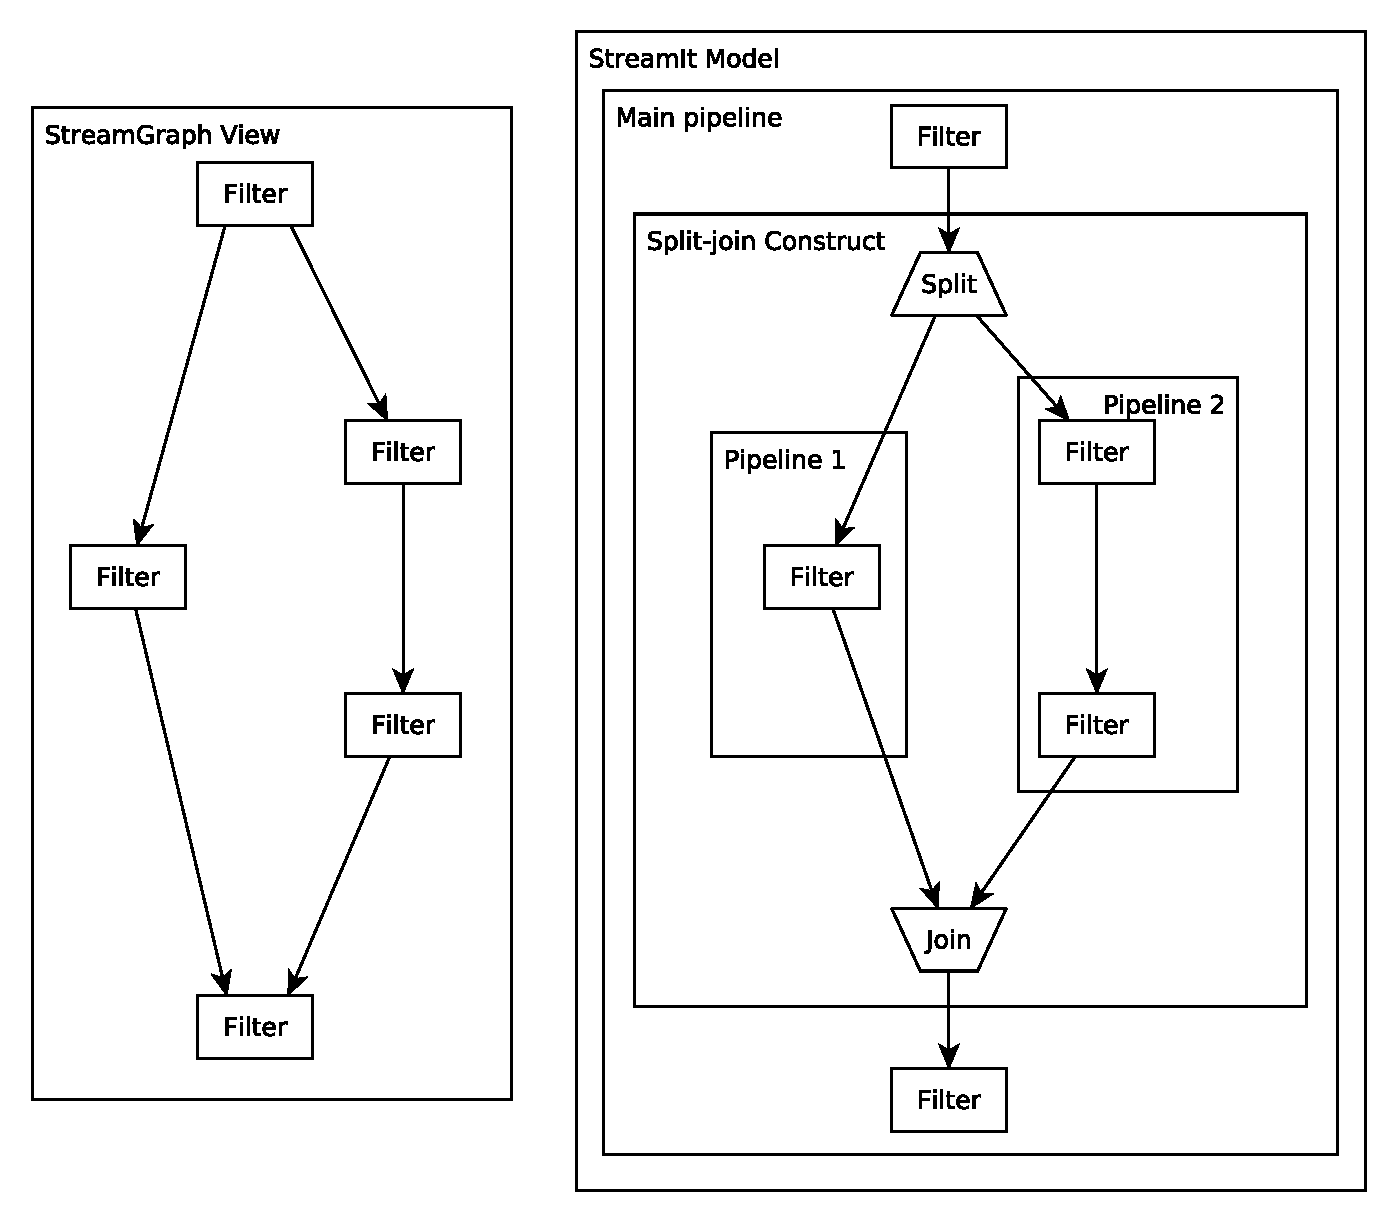
\includegraphics[width=0.8\textwidth]{StreamGraphToStreamIt}
	\caption{Example of StreamGraph to StreamIt conversion}
	\label{fig_StreamGraph_To_StreamIt}
\end{figure*}


\subsubsection{Parameter}
\noindent The Parameter class is an approximation of the way parameters are
handled in the StreamIt language. Parameters are an exception in the sense that
they are not topological constructs. In the visible graph they are represented
by nodes. Parameters do not reference other CodeObjects or filters. They only
are referenced from other objects (filters or CodeObjects). Every parameter as a
CodeObject exists exactly once.\\
For better readability in the StreamIt source file the parameters are written as
global variables in the main pipeline and are passed through to the other code
objects.\\

\subsubsection{Pipeline}
\noindent Every StreamIt program contains at least one pipeline, the main
pipeline, in which all other constructs and filters are placed. A pipeline 
CodeObject stores the objects in the order in which a data packet in StreamIt 
will be processed. These objects may be other CodeObjects like split-join 
constructs or filters. If the need for a split-join construct is detected 
while creating the pipeline a split-join construct is created. When the 
creation is complete the pipeline continues its creation and eventually 
returns.\\
Pipelines encompass the maximum possible amount of nodes to minimize the 
amount of needed pipelines and with that minimizes the amount of code 
that has to be generated. An example of a pipeline can be seen in fig. 
\ref{fig_Pipeline}.\\

\subsubsection{SplitJoin}
\noindent Split-join constructs are the most obvious parallel construct in the
StreamIt language. A split-join construct has at least two parallel paths. Every
path in a split-join is modeled as a pipeline. As such when a split-join is
created for every path the creation of a pipeline is started. In StreamIt it is
not necessary to create a pipeline if there is exactly one filter on a path
between a split-join pair. StreamGraph creates a pipeline on every path of a
split-join pair for the sake of convenience. The approach to generate a
pipeline in every case should not increase the execution time significantly and
does not change the order of execution. Because of these reasons it was decided
to not include the feature to only create pipelines in split-join constructs
when strictly necessary.\\
\\
The generation of split-joines is relatively easy as long as the graph is compatible
(for StreamIt compatibility see \ref{StreamItTopology}). As soon as the graph is not 
StreamIt compatible it becomes increasingly difficult to detect and mend. Simple 
mending methods like copying the node of a cross-connection between paths of a 
split-join is only possible if the nodes or filters are stateless. Since 
statelessness and requirements of other mending methods can only be ascertained 
through parsing and checking of the code from the respective constructs and is beyond 
the scope of this project, mending is not included in the current version of StreamGraph.\\
\\
StreamGraph does not support specific orders of execution for paths in a split-join 
construct. That means, that at the time of the first processing of the paths a specific
but random order is established. This order is then the order in which these paths will 
be processed for the whole code generation but it may be different between different
executions of the code generation.\\
A simple example of a split join is shown in fig. \ref{fig_Split_Join}.\\


\subsection{Code generation}
\noindent The code generation as a first step generates the code for every
filter in the graph. This is made possible, because filters are the basic
modules of StreamIt and due to the fact that every meaningful StreamIt program
has at least a Pipeline. As such StreamIt as a language does not allow programs
consisting only of filters because without a pipeline no connection between
these filters can be made (see \ref{StreamItTopology} for further
explanation). \\
The reasons behind generating filters at first are that in this 
way it is not possible to 'forget' a filter and if a filter is generated that 
is not needed in the execution of the program it does no harm. Second it 
simplifies the later utilization in the topological constructs, since these 
only need the name of the component and not the complete code.\\

After generating all filters the code generation continues with the main
CodeObject which is a pipeline. While generating the code of a topological
construct (a pipeline or a split-join-pair) it may be necessary to generate the
code of another such topological construct since it is a part of the first
construct. In that case the code generation of the current construct is paused
and the code generation of the contained construct is started. By the time the
code generation of the contained construct is finished the code generation of
the containing construct is continued.\\

The code generation arranges filters and topological constructs according to
their type. Thus a StreamGraph output file first lists all filters, then all
pipelines and last all split-join constructs.\\

\subsection{Improvment and Extension}



\section{Installation and Setup}



\section{Developer documentation}
\noindent In this section you can find in depth documentation to the different
parts of the StreamGraph project.
\subsection{View}



\subsection{Model}



\subsection{GraphCompat}



\subsection{Code generation}

% An example of a floating figure using the graphicx package.
%\begin{figure}[!t]
%\centering
%\includegraphics[width=2.5in]{myfigure}
%\caption{Simulation results for the network.}
%\label{fig_sim}
%\end{figure}

% An example of a double column floating figure using two subfigures.
% (The subfig.sty package must be loaded for this to work.)
%\begin{figure*}[!t]
%\centering
%\subfloat[Case I]{\includegraphics[width=2.5in]{box}%
%\label{fig_first_case}}
%\hfil
%\subfloat[Case II]{\includegraphics[width=2.5in]{box}%
%\label{fig_second_case}}
%\caption{Simulation results for the network.}
%\label{fig_sim}
%\end{figure*}

% An example of a floating table.
%\begin{table}[!t]
%% increase table row spacing, adjust to taste
%\renewcommand{\arraystretch}{1.3}
% if using array.sty, it might be a good idea to tweak the value of
% \extrarowheight as needed to properly center the text within the cells
%\caption{An Example of a Table}
%\label{table_example}
%\centering
%% Some packages, such as MDW tools, offer better commands for making tables
%% than the plain LaTeX2e tabular which is used here.
%\begin{tabular}{|c||c|}
%\hline
%One & Two\\
%\hline
%Three & Four\\
%\hline
%\end{tabular}
%\end{table}

\section{Conclusion}
\noindent The conclusion goes here.

\appendices


% use section* for acknowledgment
\section*{Acknowledgment}


\noindent The authors would like to thank...

\ifCLASSOPTIONcaptionsoff
  \newpage
\fi

\begin{thebibliography}{1}

\bibitem{streamIt}
William~Thies, Michael~Karczmarek, and Saman~Amarasinghe, \emph{StreamIt: A Language for Streaming Applications},\hskip 1em plus
  0.5em minus 0.4em\relax Laboratory for Computer Science, Massachusetts Institute of Technology, Cambridge, MA 02139.
\bibitem{GTK2EXMindMapView}
\url{http://search.cpan.org/~hemlock/Gtk2-Ex-MindMapView-0.000001/lib/Gtk2/Ex/MindMapView.pm}
\end{thebibliography}

% that's all folks
\end{document}
